%===============================================================================
% LaTeX sjabloon voor de bachelorproef toegepaste informatica aan HOGENT
% Meer info op https://github.com/HoGentTIN/latex-hogent-report
%===============================================================================

\documentclass[dutch,dit,thesis]{hogentreport}

\usepackage{float}
\usepackage{pgfgantt}
\usepackage{wrapfig}

% TODO:
% - If necessary, replace the option `dit`' with your own department!
%   Valid entries are dbo, dbt, dgz, dit, dlo, dog, dsa, soa
% - If you write your thesis in English (remark: only possible after getting
%   explicit approval!), remove the option "dutch," or replace with "english".

\usepackage{lipsum} % For blind text, can be removed after adding actual content

%% Pictures to include in the text can be put in the graphics/ folder
\graphicspath{{../graphics/}}

%% For source code highlighting, requires pygments to be installed
%% Compile with the -shell-escape flag!
%% \usepackage[chapter]{minted}
%% If you compile with the make_thesis.{bat,sh} script, use the following
%% import instead:
\usepackage[chapter,outputdir=../output]{minted}
\usemintedstyle{solarized-light}

%% Formatting for minted environments.
\setminted{%
    autogobble,
    frame=lines,
    breaklines,
    linenos,
    tabsize=4
}

%% Ensure the list of listings is in the table of contents
\renewcommand\listoflistingscaption{%
    \IfLanguageName{dutch}{Lijst van codefragmenten}{List of listings}
}
\renewcommand\listingscaption{%
    \IfLanguageName{dutch}{Codefragment}{Listing}
}
\renewcommand*\listoflistings{%
    \cleardoublepage\phantomsection\addcontentsline{toc}{chapter}{\listoflistingscaption}%
    \listof{listing}{\listoflistingscaption}%
}

% Other packages not already included can be imported here

%%---------- Document metadata -------------------------------------------------
% TODO: Replace this with your own information
\author{Xander Van der Steichel}
\supervisor{Dhr. S. Verschraege}
\cosupervisor{Dhr. A. Boel}
\title
{Automatisering van het orderproces van website naar 3D-geprinte producten}

\academicyear{\advance\year by -1 \the\year--\advance\year by 1 \the\year}
\examperiod{1}
\degreesought{\IfLanguageName{dutch}{Professionele bachelor in de toegepaste informatica}{Bachelor of applied computer science}}
\partialthesis{false} %% To display 'in partial fulfilment'
%\institution{Internshipcompany BVBA.}

%% Add global exceptions to the hyphenation here
\hyphenation{back-slash}

%% The bibliography (style and settings are  found in hogentthesis.cls)
\addbibresource{bachproef.bib}            %% Bibliography file
\addbibresource{../voorstel/voorstel.bib} %% Bibliography research proposal
\defbibheading{bibempty}{}

%% Prevent empty pages for right-handed chapter starts in twoside mode
\renewcommand{\cleardoublepage}{\clearpage}

\renewcommand{\arraystretch}{1.2}

%% Content starts here.
\begin{document}

%---------- Front matter -------------------------------------------------------

\frontmatter

\hypersetup{pageanchor=false} %% Disable page numbering references
%% Render a Dutch outer title page if the main language is English
\IfLanguageName{english}{%
    %% If necessary, information can be changed here
    \degreesought{Professionele Bachelor toegepaste informatica}%
    \begin{otherlanguage}{dutch}%
       \maketitle%
    \end{otherlanguage}%
}{}

%% Generates title page content
\maketitle
\hypersetup{pageanchor=true}


%%=============================================================================
%% Voorwoord
%%=============================================================================

\chapter*{\IfLanguageName{dutch}{Woord vooraf}{Preface}}%
\label{ch:voorwoord}

%% TODO:
%% Het voorwoord is het enige deel van de bachelorproef waar je vanuit je
%% eigen standpunt (``ik-vorm'') mag schrijven. Je kan hier bv. motiveren
%% waarom jij het onderwerp wil bespreken.
%% Vergeet ook niet te bedanken wie je geholpen/gesteund/... heeft

\lipsum[1-2]
%%=============================================================================
%% Samenvatting
%%=============================================================================

% TODO: De "abstract" of samenvatting is een kernachtige (~ 1 blz. voor een
% thesis) synthese van het document.
%
% Een goede abstract biedt een kernachtig antwoord op volgende vragen:
%
% 1. Waarover gaat de bachelorproef?
% 2. Waarom heb je er over geschreven?
% 3. Hoe heb je het onderzoek uitgevoerd?
% 4. Wat waren de resultaten? Wat blijkt uit je onderzoek?
% 5. Wat betekenen je resultaten? Wat is de relevantie voor het werkveld?
%
% Daarom bestaat een abstract uit volgende componenten:
%
% - inleiding + kaderen thema
% - probleemstelling
% - (centrale) onderzoeksvraag
% - onderzoeksdoelstelling
% - methodologie
% - resultaten (beperk tot de belangrijkste, relevant voor de onderzoeksvraag)
% - conclusies, aanbevelingen, beperkingen
%
% LET OP! Een samenvatting is GEEN voorwoord!

%%---------- Nederlandse samenvatting -----------------------------------------
%
% TODO: Als je je bachelorproef in het Engels schrijft, moet je eerst een
% Nederlandse samenvatting invoegen. Haal daarvoor onderstaande code uit
% commentaar.
% Wie zijn bachelorproef in het Nederlands schrijft, kan dit negeren, de inhoud
% wordt niet in het document ingevoegd.

\IfLanguageName{english}{%
\selectlanguage{dutch}
\chapter*{Samenvatting}
\lipsum[1-4]
\selectlanguage{english}
}{}

%%---------- Samenvatting -----------------------------------------------------
% De samenvatting in de hoofdtaal van het document

\chapter*{\IfLanguageName{dutch}{Samenvatting}{Abstract}}

\lipsum[1-4]


%---------- Inhoud, lijst figuren, ... -----------------------------------------

\tableofcontents

% In a list of figures, the complete caption will be included. To prevent this,
% ALWAYS add a short description in the caption!
%
%  \caption[short description]{elaborate description}
%
% If you do, only the short description will be used in the list of figures

\listoffigures

% If you included tables and/or source code listings, uncomment the appropriate
% lines.
\listoftables

\listoflistings

% Als je een lijst van afkortingen of termen wil toevoegen, dan hoort die
% hier thuis. Gebruik bijvoorbeeld de ``glossaries'' package.
% https://www.overleaf.com/learn/latex/Glossaries

%---------- Kern ---------------------------------------------------------------

\mainmatter{}

% De eerste hoofdstukken van een bachelorproef zijn meestal een inleiding op
% het onderwerp, literatuurstudie en verantwoording methodologie.
% Aarzel niet om een meer beschrijvende titel aan deze hoofdstukken te geven of
% om bijvoorbeeld de inleiding en/of stand van zaken over meerdere hoofdstukken
% te verspreiden!

%%=============================================================================
%% Inleiding
%%=============================================================================

\chapter{\IfLanguageName{dutch}{Inleiding}{Introduction}}%
\label{ch:inleiding}

In de huidige digitale economie wordt automatisering steeds belangrijker om efficiënter te werkt te gaan en menselijke fouten te beperken. Binnen de e-commerce sector met 3D-printing is een gestroomlijnde workflow van belang om bestellingen snel en accuraat te verwerken. Deze bachelorproef richt zich op de automatisering van het orderproces voor 3D-geprinte producten. Het doel is om een pipeline te ontwikkelen in Python die een Shopify-API koppelt aan de API van Bambu Studio. Hiermee wordt een geautomatiseerde workflow mogelijk gemaakt waarbij bestellingen na ontvangst automatisch worden verwerkt en doorgestuurd naar de 3D-printer.

%De inleiding moet de lezer net genoeg informatie verschaffen om het onderwerp te begrijpen en in te zien waarom de onderzoeksvraag de moeite waard is om te onderzoeken. In de inleiding ga je literatuurverwijzingen beperken, zodat de tekst vlot leesbaar blijft. Je kan de inleiding verder onderverdelen in secties als dit de tekst verduidelijkt. Zaken die aan bod kunnen komen in de inleiding~\autocite{Pollefliet2011}:

%\begin{itemize}
 % \item context, achtergrond
 % \item afbakenen van het onderwerp
 % \item verantwoording van het onderwerp, methodologie
 % \item probleemstelling
 % \item onderzoeksdoelstelling
 % \item onderzoeksvraag
 % \item \ldots
%\end{itemize}

\section{\IfLanguageName{dutch}{Probleemstelling}{Problem Statement}}%
\label{sec:probleemstelling}

Momenteel vereisen veel webshops die 3D-geprinte producten aanbieden een handmatige verwerking van bestellingen. Dit proces is tijdrovend en foutgevoelig. Door de koppeling van Shopify met Bambu Studio te automatiseren, kan het orderproces efficiënter verlopen, wat resulteert in snellere leveringstijden en minder fysieke opdrachten. Dit onderzoek richt zich op het ontwikkelen en implementeren van een oplossing die deze automatisering mogelijk maakt.

%Uit je probleemstelling moet duidelijk zijn dat je onderzoek een meerwaarde heeft voor een concrete doelgroep. De doelgroep moet goed gedefinieerd en afgelijnd zijn. Doelgroepen als ``bedrijven,'' ``KMO's'', systeembeheerders, enz.~zijn nog te vaag. Als je een lijstje kan maken van de personen/organisaties die een meerwaarde zullen vinden in deze bachelorproef (dit is eigenlijk je steekproefkader), dan is dat een indicatie dat de doelgroep goed gedefinieerd is. Dit kan een enkel bedrijf zijn of zelfs één persoon (je co-promotor/opdrachtgever).

\section{\IfLanguageName{dutch}{Onderzoeksvraag}{Research question}}%
\label{sec:onderzoeksvraag}

De centrale onderzoeksvraag van deze bachelorproef luidt: "Hoe kan een Python-gebaseerde pipeline worden ontwikkeld om het orderproces van een Shopify-webshop te automatiseren met behulp van de Bambu Studio API?" Deze vraag wordt verder opgesplitst in deelvragen zoals:

\begin{itemize}
    \item Welke functionaliteiten biedt de Shopify API voor orderverwerking?
    \item Hoe kan de Bambu Studio API orders efficiënt verwerken?
    \item Welke uitdagingen en beperkingen zijn er bij de implementatie van een geautomatiseerde pipeline?
    \item Welke bestaande pipelines kunnen worden vergeleken om de meest geschikte aanpak te bepalen?
\end{itemize}

%Wees zo concreet mogelijk bij het formuleren van je onderzoeksvraag. Een onderzoeksvraag is trouwens iets waar nog niemand op dit moment een antwoord heeft (voor zover je kan nagaan). Het opzoeken van bestaande informatie (bv. ``welke tools bestaan er voor deze toepassing?'') is dus geen onderzoeksvraag. Je kan de onderzoeksvraag verder specifiëren in deelvragen. Bv.~als je onderzoek gaat over performantiemetingen, dan 

\section{\IfLanguageName{dutch}{Onderzoeksdoelstelling}{Research objective}}%
\label{sec:onderzoeksdoelstelling}

Het doel van deze bachelorproef is het ontwikkelen van een proof-of-concept dat de orderverwerking van een Shopify-webshop volledig automatiseert via een koppeling met de Bambu Studio API. Een belangrijk onderdeel van dit onderzoek is het vergelijken van verschillende pipelines om de meest efficiënte en betrouwbare oplossing te bepalen. Het succes van deze implementatie wordt beoordeeld aan de hand van criteria zoals betrouwbaarheid, verwerkingssnelheid en foutreductie.

%Wat is het beoogde resultaat van je bachelorproef? Wat zijn de criteria voor succes? Beschrijf die zo concreet mogelijk. Gaat het bv.\ om een proof-of-concept, een prototype, een verslag met aanbevelingen, een vergelijkende studie, enz.

\section{\IfLanguageName{dutch}{Opzet van deze bachelorproef}{Structure of this bachelor thesis}}%
\label{sec:opzet-bachelorproef}

% Het is gebruikelijk aan het einde van de inleiding een overzicht te
% geven van de opbouw van de rest van de tekst. Deze sectie bevat al een aanzet
% die je kan aanvullen/aanpassen in functie van je eigen tekst.

De rest van deze bachelorproef is als volgt opgebouwd:

In Hoofdstuk~\ref{ch:stand-van-zaken} wordt een overzicht gegeven van de stand van zaken binnen het onderzoeksdomein, op basis van een literatuurstudie.

In Hoofdstuk~\ref{ch:methodologie} wordt de methodologie toegelicht en worden de gebruikte onderzoekstechnieken besproken om een antwoord te kunnen formuleren op de onderzoeksvragen.

% TODO: Vul hier aan voor je eigen hoofstukken, één of twee zinnen per hoofdstuk

In Hoofdstuk~\ref{ch:conclusie}, tenslotte, wordt de conclusie gegeven en een antwoord geformuleerd op de onderzoeksvragen. Daarbij wordt ook een aanzet gegeven voor toekomstig onderzoek binnen dit domein.
\chapter{\IfLanguageName{dutch}{Stand van zaken}{State of the art}}%
\label{ch:stand-van-zaken}

% Tip: Begin elk hoofdstuk met een paragraaf inleiding die beschrijft hoe
% dit hoofdstuk past binnen het geheel van de bachelorproef. Geef in het
% bijzonder aan wat de link is met het vorige en volgende hoofdstuk.

% Pas na deze inleidende paragraaf komt de eerste sectiehoofding.

Dit hoofdstuk bevat je literatuurstudie. De inhoud gaat verder op de inleiding, maar zal het onderwerp van de bachelorproef *diepgaand* uitspitten. De bedoeling is dat de lezer na lezing van dit hoofdstuk helemaal op de hoogte is van de huidige stand van zaken (state-of-the-art) in het onderzoeksdomein. Iemand die niet vertrouwd is met het onderwerp, weet nu voldoende om de rest van het verhaal te kunnen volgen, zonder dat die er nog andere informatie moet over opzoeken \autocite{Pollefliet2011}.

Je verwijst bij elke bewering die je doet, vakterm die je introduceert, enz.\ naar je bronnen. In \LaTeX{} kan dat met het commando \texttt{$\backslash${textcite\{\}}} of \texttt{$\backslash${autocite\{\}}}. Als argument van het commando geef je de ``sleutel'' van een ``record'' in een bibliografische databank in het Bib\LaTeX{}-formaat (een tekstbestand). Als je expliciet naar de auteur verwijst in de zin (narratieve referentie), gebruik je \texttt{$\backslash${}textcite\{\}}. Soms is de auteursnaam niet expliciet een onderdeel van de zin, dan gebruik je \texttt{$\backslash${}autocite\{\}} (referentie tussen haakjes). Dit gebruik je bv.~bij een citaat, of om in het bijschrift van een overgenomen afbeelding, broncode, tabel, enz. te verwijzen naar de bron. In de volgende paragraaf een voorbeeld van elk.

\textcite{Knuth1998} schreef een van de standaardwerken over sorteer- en zoekalgoritmen. Experten zijn het erover eens dat cloud computing een interessante opportuniteit vormen, zowel voor gebruikers als voor dienstverleners op vlak van informatietechnologie~\autocite{Creeger2009}.

Let er ook op: het \texttt{cite}-commando voor de punt, dus binnen de zin. Je verwijst meteen naar een bron in de eerste zin die erop gebaseerd is, dus niet pas op het einde van een paragraaf.

\begin{figure}
  \centering
  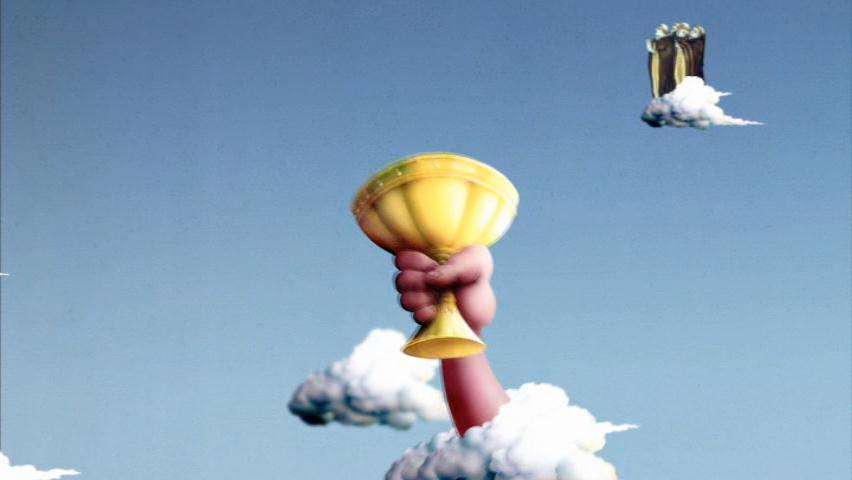
\includegraphics[width=0.8\textwidth]{grail.jpg}
  \caption[Voorbeeld figuur.]{\label{fig:grail}Voorbeeld van invoegen van een figuur. Zorg altijd voor een uitgebreid bijschrift dat de figuur volledig beschrijft zonder in de tekst te moeten gaan zoeken. Vergeet ook je bronvermelding niet!}
\end{figure}

\begin{listing}
  \begin{minted}{python}
    import pandas as pd
    import seaborn as sns

    penguins = sns.load_dataset('penguins')
    sns.relplot(data=penguins, x="flipper_length_mm", y="bill_length_mm", hue="species")
  \end{minted}
  \caption[Voorbeeld codefragment]{Voorbeeld van het invoegen van een codefragment.}
\end{listing}

\lipsum[7-20]

\begin{table}
  \centering
  \begin{tabular}{lcr}
    \toprule
    \textbf{Kolom 1} & \textbf{Kolom 2} & \textbf{Kolom 3} \\
    $\alpha$         & $\beta$          & $\gamma$         \\
    \midrule
    A                & 10.230           & a                \\
    B                & 45.678           & b                \\
    C                & 99.987           & c                \\
    \bottomrule
  \end{tabular}
  \caption[Voorbeeld tabel]{\label{tab:example}Voorbeeld van een tabel.}
\end{table}


%%=============================================================================
%% Methodologie
%%=============================================================================


\chapter{\IfLanguageName{dutch}{Methodologie}{Methodology}}%
\label{ch:methodologie}

%% TODO: In dit hoofstuk geef je een korte toelichting over hoe je te werk bent
%% gegaan. Verdeel je onderzoek in grote fasen, en licht in elke fase toe wat
%% de doelstelling was, welke deliverables daar uit gekomen zijn, en welke
%% onderzoeksmethoden je daarbij toegepast hebt. Verantwoord waarom je
%% op deze manier te werk gegaan bent.
%% 
%% Voorbeelden van zulke fasen zijn: literatuurstudie, opstellen van een
%% requirements-analyse, opstellen long-list (bij vergelijkende studie),
%% selectie van geschikte tools (bij vergelijkende studie, "short-list"),
%% opzetten testopstelling/PoC, uitvoeren testen en verzamelen
%% van resultaten, analyse van resultaten, ...
%%
%% !!!!! LET OP !!!!!
%%
%% Het is uitdrukkelijk NIET de bedoeling dat je het grootste deel van de corpus
%% van je bachelorproef in dit hoofstuk verwerkt! Dit hoofdstuk is eerder een
%% kort overzicht van je plan van aanpak.
%%
%% Maak voor elke fase (behalve het literatuuronderzoek) een NIEUW HOOFDSTUK aan
%% en geef het een gepaste titel.

Het doel van dit onderzoek is het identificeren van de meest geschikte pipeline voor de automatisering van het orderproces van een website naar 3D-geprinte producten. Dit proces zal iteratief verlopen, met fasen die zich richten op onderzoek, evaluatie, en prototyping. Elke fase heeft specifieke doelstellingen, deliverables en deadlines. Regelmatige feedback van de Co-promotor zal worden gezocht om de voortgang te evalueren en bij te sturen waar nodig. Ook is het de bedoeling dat deze pipeline zal draaien op Mac en Windows.
\vspace{2em}

\textbf{Fase 1: Literatuurstudie}\\
\textbf{(Deadline: 07 maart 2025)}\\\\
In deze fase wordt er literatuuronderzoek gedaan naar bestaande oplossingen en pipelines die gebruikt kunnen worden voor de automatisering van het orderproces. Dit omvat een analyse van tools zoals Python, integraties met de Shopify API, en printbeheer API's zoals Bambu Studio. De deliverable voor deze fase is een lijst met mogelijke pipelines en tools die geschikt zouden kunnen zijn voor dit project, inclusief voor- en nadelen van elke optie.
\vspace{2em}

\textbf{Fase 2: Proof-of-Concept (PoC)}\\
\textbf{(Deadline: 4 april 2025)}\\\\
Op basis van de literatuurstudie worden meerdere pipelines geselecteerd en getest door een PoC op te zetten voor elke gekozen oplossing. Dit zal helpen om de haalbaarheid van de verschillende pipelines te testen. De PoC zal een order ontvangen via de Shopify API en doorsturen naar de Bambu Studio API. De technische haalbaarheid van elke pipeline wordt geëvalueerd om te bepalen welke het beste presteert.
\vspace{1em}

\textbf{Fase 3: Testen van de Pipelines en Prestatieanalyse}\\
\textbf{(Deadline: 18 April 2025)}\\\\
In deze fase worden de geselecteerde pipelines verder getest. Dit houdt in dat de pipelines onder verschillende belasting- en stressomstandigheden worden getest, zoals het verwerken van meerdere orders tegelijk. Daarnaast wordt er gekeken naar foutafhandelingsmechanismen en de stabiliteit van de integratie met de APIs. Enkele testscenario's omvatten: 
\begin{itemize}
    \item Wat gebeurt er als een bestand mislukt bij het verzenden?
    \item Wat gebeurt er als de printer zonder stroom valt?
    \item Wat gebeurt er bij een printfout?
    \item Hoe wordt het beëindigen van het printproces afgehandeld? 
\end{itemize}
\vspace{1em}

\textbf{Fase 4: Keuze van de Beste Pipeline en Optimalisatie}\\
\textbf{(Deadline: 25 april 2025)}\\\\
Na de uitvoerige tests wordt de beste pipeline geselecteerd op basis van prestaties, fouttolerantie en integratiegemak. In deze fase worden eventuele optimalisaties doorgevoerd en wordt de gekozen oplossing verder verfijnd voor de uiteindelijke implementatie.

\vspace{1em}
\textbf{Dit is de verwachte lijst van Tools:}\\
\begin{itemize}
    \item Python: voor het bouwen van de pipeline en het uitvoeren van API-aanroepen.
    \item Shopify API en Bambu Studio API: om orders te ontvangen en printopdrachten door te sturen.
    \item GitHub: voor versiebeheer van de code en documentatie.
    \item Postman: voor het testen van API-aanroepen tijdens de ontwikkeling.
    \item 3D-printer Bambu Lab X1C: voor het fysiek testen van het printproces.
    \item Verschillende pipelinetools: voor het opzetten en automatiseren van de integratie tussen de verschillende onderdelen van het systeem.
\end{itemize}

\vspace{1em}
\textbf{Dit is de verwachte lijst van functionele vereisten voor de applicatie:}\\
\begin{itemize}
    \item \textbf{MUST}
    \begin{itemize}
        \item Order moet kunnen opgehaald worden  via de API.
        \item Juiste file moet kunnen opgehaald worden.
        \item Printopdracht moet kunnen gestart worden via de API.
    \end{itemize}
    \item \textbf{SHOULD}
    \begin{itemize}
        \item Communicatie naar eigenaar dat print gelsaagd is.
    \end{itemize}
    \item \textbf{COULD}
    \begin{itemize}
        \item Als meerdere orders binnenkomen deze samen plaatsen op het printbed indien mogelijk.
    \end{itemize}
\end{itemize}

\vspace{1em}
\textbf{Planning en deliverables}

\begin{itemize}
    \item Gemaakte flowchart
    
    \begin{figure}[H]  % Use [H] to prevent floating
        \centering
        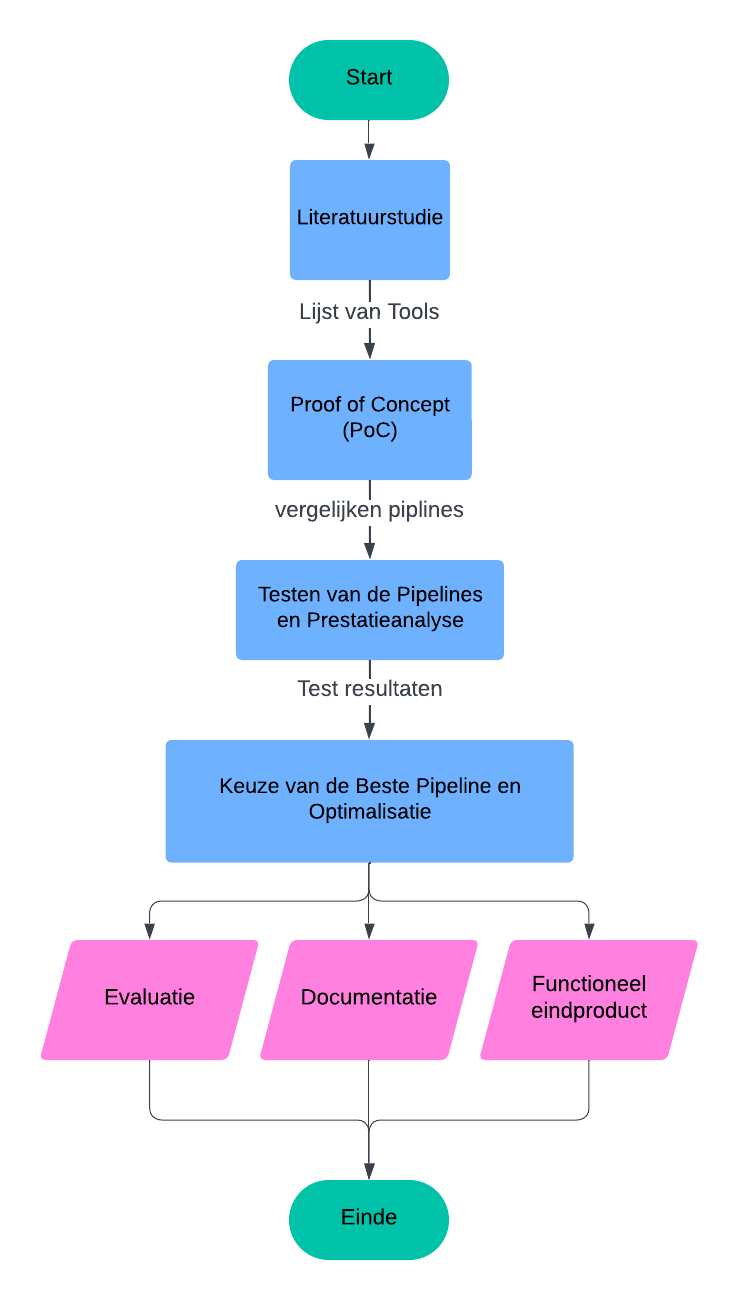
\includegraphics[width=0.5\textwidth]{Flowchart.png}  % Adjust width if necessary
        \caption{Flowchart van verschillende fasen en deliverables van de bachelorproef.}
        \label{fig:flowchart}  % Label for referencing
    \end{figure}
    
    \item Gemaakte Gantt chart.
    
    % Second figure: The Gantt Chart
    \begin{figure}[H]  % Use [H] to prevent floating
        \centering
        \resizebox{\textwidth}{!}{%
            \begin{ganttchart}[
                vgrid,
                hgrid,
                x unit=0.1cm,
                time slot format=isodate,
                compress calendar
                ]{2025-02-01}{2025-05-30}
                
                \gantttitlecalendar{year, month=name} \\
                
                % Fase 1: Literatuurstudie
                \ganttbar[
                progress=100,
                name=litstudie
                ]{Fase 1: Literatuurstudie}{2025-02-01}{2025-02-20} \\
                
                % Fase 2: Proof of Concept (PoC)
                \ganttbar[
                progress=0,
                name=poc
                ]{Fase 2: Proof-of-Concept}{2025-02-21}{2025-04-04} \\
                
                % Fase 3: Experimenten en Testen
                \ganttbar[
                progress=0,
                name=testen
                ]{Fase 3: Testen van de Pipelines en Prestatieanalyse}{2025-04-05}{2025-04-18} \\
                
                % Fase 4: Iteratieve Ontwikkeling en Optimalisatie
                \ganttbar[
                progress=0,
                name=optimalisatie
                ]{Fase 4: Keuze van de Beste Pipeline en Optimalisatie}{2025-04-19}{2025-04-25} \\
                
            \end{ganttchart}
        }
        \caption{Project Planning Gantt Chart}
        \label{fig:ganttchart}  % Label for referencing
    \end{figure}
\end{itemize}




% Voeg hier je eigen hoofdstukken toe die de ``corpus'' van je bachelorproef
% vormen. De structuur en titels hangen af van je eigen onderzoek. Je kan bv.
% elke fase in je onderzoek in een apart hoofdstuk bespreken.

%\input{...}
%\input{...}
%...

%%=============================================================================
%% Conclusie
%%=============================================================================

\chapter{Conclusie}%
\label{ch:conclusie}

% TODO: Trek een duidelijke conclusie, in de vorm van een antwoord op de
% onderzoeksvra(a)g(en). Wat was jouw bijdrage aan het onderzoeksdomein en
% hoe biedt dit meerwaarde aan het vakgebied/doelgroep? 
% Reflecteer kritisch over het resultaat. In Engelse teksten wordt deze sectie
% ``Discussion'' genoemd. Had je deze uitkomst verwacht? Zijn er zaken die nog
% niet duidelijk zijn?
% Heeft het onderzoek geleid tot nieuwe vragen die uitnodigen tot verder 
%onderzoek?

Dit bachelorproject onderzocht hoe een e-commerce platform zoals Shopify automatisch fysieke producten kan laten printen via een 3D-printer, zonder handmatige tussenkomst. Concreet werd onderzocht hoe een CI/CD-pipeline, zoals Jenkins, GitHub Actions of GitLab CI, gebruikt kan worden als brug tussen een webshop en een 3D-printer die aangestuurd wordt via Moonraker.

Om dit te realiseren werden drie proof-of-concepts (PoC's) uitgewerkt:

\begin{itemize}
    \item \textbf{PoC 1} toonde aan dat Jenkins succesvol 3D-printtaken kan starten op basis van een Shopify-webhook. De pipeline uploadt G-code bestanden, start de printerqueue en wacht actief tot de print voltooid is.
    
    \item \textbf{PoC 2} bewees dat GitHub Actions ook geschikt is voor deze automatisatie, mits een externe tussenlaag (zoals een Express.js server) de webhooks opvangt en doorstuurt naar GitHub.
    
    \item \textbf{PoC 3} exploreerde de mogelijkheden met GitLab CI, met een focus op eenvoud en betere integratie-opties. GitLab toont gelijkaardige flexibiliteit.
\end{itemize}

De meest mature oplossing op technisch vlak was \textbf{PoC 1}, die het volledige proces van bestelling tot geprinte output afhandelt. Dankzij Jenkins' configuratie om builds niet parallel uit te voeren (\texttt{Do not allow concurrent builds}), en wordt elke bestelling in volgorde verwerkt. De pipeline wacht per product actief tot de print afgerond is, waardoor betrouwbaarheid en traceerbaarheid gegarandeerd zijn.

\section*{Bijdrage aan het domein}

Het project toont aan dat CI/CD-tools niet enkel nuttig zijn voor softwaredeployments, maar ook als coördinatieplatform kunnen dienen voor fysieke processen zoals 3D-printing. Deze benadering is relatief ongezien, en biedt een laagdrempelige automatisatie-oplossing aan voor kleine ondernemingen die geen toegang hebben tot complexe productielijnen of gespecialiseerde MES-software.

\section*{Kritische reflectie}

De pipelines functioneren stabiel en robuust, maar vereisen wel enige technische setup, vooral qua netwerkinstellingen (zoals ngrok of port forwarding). In een productiecontext zou een meer beveiligde oplossing vereist zijn.

Ook blijft foutafhandeling aan de printerkant een uitdaging. Hoewel de pipeline printerfouten detecteert via de Moonraker API, kunnen problemen zoals mechanische falen of slecht gelevelde bedden enkel deels worden opgevangen.

\section*{Vervolgonderzoek}

Er zijn meerdere opportuniteiten voor vervolgonderzoek:

\begin{itemize}
    \item Integratie met meerdere printers tegelijk, en load balancing.
    \item Integratie met order- en voorraadbeheer (bv. automatisch printen bij lage stock).
    \item Meer verfijnde foutafhandeling en recovery-opties (bv. notificaties via mail of Discord).
    \item Een visuele interface om printstatussen op te volgen.
\end{itemize}

\bigskip

Tot slot toont dit project aan dat zelfs met bestaande tools zoals Jenkins en enkele scripts, een betrouwbare, flexibele en schaalbare printautomatisatie mogelijk is – een brug tussen digitale bestellingen en fysieke productie.




%---------- Bijlagen -----------------------------------------------------------

\appendix

\chapter{Onderzoeksvoorstel}

Het onderwerp van deze bachelorproef is gebaseerd op een onderzoeksvoorstel dat vooraf werd beoordeeld door de promotor. Dat voorstel is opgenomen in deze bijlage.

%% TODO: 
%\section*{Samenvatting}

% Kopieer en plak hier de samenvatting (abstract) van je onderzoeksvoorstel.

% Verwijzing naar het bestand met de inhoud van het onderzoeksvoorstel
%---------- Inleiding ---------------------------------------------------------

% TODO: Is dit voorstel gebaseerd op een paper van Research Methods die je
% vorig jaar hebt ingediend? Heb je daarbij eventueel samengewerkt met een
% andere student?
% Zo ja, haal dan de tekst hieronder uit commentaar en pas aan.

%\paragraph{Opmerking}

% Dit voorstel is gebaseerd op het onderzoeksvoorstel dat werd geschreven in het
% kader van het vak Research Methods dat ik (vorig/dit) academiejaar heb
% uitgewerkt (met medesturent VOORNAAM NAAM als mede-auteur).
% 

\section{Inleiding}%
\label{sec:inleiding}

Waarover zal je bachelorproef gaan? Introduceer het thema en zorg dat volgende zaken zeker duidelijk aanwezig zijn:

\begin{itemize}
  \item kaderen thema
  \item de doelgroep
  \item de probleemstelling en (centrale) onderzoeksvraag
  \item de onderzoeksdoelstelling
\end{itemize}

Denk er aan: een typische bachelorproef is \textit{toegepast onderzoek}, wat betekent dat je start vanuit een concrete probleemsituatie in bedrijfscontext, een \textbf{casus}. Het is belangrijk om je onderwerp goed af te bakenen: je gaat voor die \textit{ene specifieke probleemsituatie} op zoek naar een goede oplossing, op basis van de huidige kennis in het vakgebied.

De doelgroep moet ook concreet en duidelijk zijn, dus geen algemene of vaag gedefinieerde groepen zoals \emph{bedrijven}, \emph{developers}, \emph{Vlamingen}, enz. Je richt je in elk geval op it-professionals, een bachelorproef is geen populariserende tekst. Eén specifiek bedrijf (die te maken hebben met een concrete probleemsituatie) is dus beter dan \emph{bedrijven} in het algemeen.

Formuleer duidelijk de onderzoeksvraag! De begeleiders lezen nog steeds te veel voorstellen waarin we geen onderzoeksvraag terugvinden.

Schrijf ook iets over de doelstelling. Wat zie je als het concrete eindresultaat van je onderzoek, naast de uitgeschreven scriptie? Is het een proof-of-concept, een rapport met aanbevelingen, \ldots Met welk eindresultaat kan je je bachelorproef als een succes beschouwen?

%---------- Stand van zaken ---------------------------------------------------

\section{Literatuurstudie}%
\label{sec:literatuurstudie}

Hier beschrijf je de \emph{state-of-the-art} rondom je gekozen onderzoeksdomein, d.w.z.\ een inleidende, doorlopende tekst over het onderzoeksdomein van je bachelorproef. Je steunt daarbij heel sterk op de professionele \emph{vakliteratuur}, en niet zozeer op populariserende teksten voor een breed publiek. Wat is de huidige stand van zaken in dit domein, en wat zijn nog eventuele open vragen (die misschien de aanleiding waren tot je onderzoeksvraag!)?

Je mag de titel van deze sectie ook aanpassen (literatuurstudie, stand van zaken, enz.). Zijn er al gelijkaardige onderzoeken gevoerd? Wat concluderen ze? Wat is het verschil met jouw onderzoek?

Verwijs bij elke introductie van een term of bewering over het domein naar de vakliteratuur, bijvoorbeeld~\autocite{Hykes2013}! Denk zeker goed na welke werken je refereert en waarom.

Draag zorg voor correcte literatuurverwijzingen! Een bronvermelding hoort thuis \emph{binnen} de zin waar je je op die bron baseert, dus niet er buiten! Maak meteen een verwijzing als je gebruik maakt van een bron. Doe dit dus \emph{niet} aan het einde van een lange paragraaf. Baseer nooit teveel aansluitende tekst op eenzelfde bron.

Als je informatie over bronnen verzamelt in JabRef, zorg er dan voor dat alle nodige info aanwezig is om de bron terug te vinden (zoals uitvoerig besproken in de lessen Research Methods).

% Voor literatuurverwijzingen zijn er twee belangrijke commando's:
% \autocite{KEY} => (Auteur, jaartal) Gebruik dit als de naam van de auteur
%   geen onderdeel is van de zin.
% \textcite{KEY} => Auteur (jaartal)  Gebruik dit als de auteursnaam wel een
%   functie heeft in de zin (bv. ``Uit onderzoek door Doll & Hill (1954) bleek
%   ...'')

Je mag deze sectie nog verder onderverdelen in subsecties als dit de structuur van de tekst kan verduidelijken.

%---------- Methodologie ------------------------------------------------------
\section{Methodologie}%
\label{sec:methodologie}

Hier beschrijf je hoe je van plan bent het onderzoek te voeren. Welke onderzoekstechniek ga je toepassen om elk van je onderzoeksvragen te beantwoorden? Gebruik je hiervoor literatuurstudie, interviews met belanghebbenden (bv.~voor requirements-analyse), experimenten, simulaties, vergelijkende studie, risico-analyse, PoC, \ldots?

Valt je onderwerp onder één van de typische soorten bachelorproeven die besproken zijn in de lessen Research Methods (bv.\ vergelijkende studie of risico-analyse)? Zorg er dan ook voor dat we duidelijk de verschillende stappen terug vinden die we verwachten in dit soort onderzoek!

Vermijd onderzoekstechnieken die geen objectieve, meetbare resultaten kunnen opleveren. Enquêtes, bijvoorbeeld, zijn voor een bachelorproef informatica meestal \textbf{niet geschikt}. De antwoorden zijn eerder meningen dan feiten en in de praktijk blijkt het ook bijzonder moeilijk om voldoende respondenten te vinden. Studenten die een enquête willen voeren, hebben meestal ook geen goede definitie van de populatie, waardoor ook niet kan aangetoond worden dat eventuele resultaten representatief zijn.

Uit dit onderdeel moet duidelijk naar voor komen dat je bachelorproef ook technisch voldoen\-de diepgang zal bevatten. Het zou niet kloppen als een bachelorproef informatica ook door bv.\ een student marketing zou kunnen uitgevoerd worden.

Je beschrijft ook al welke tools (hardware, software, diensten, \ldots) je denkt hiervoor te gebruiken of te ontwikkelen.

Probeer ook een tijdschatting te maken. Hoe lang zal je met elke fase van je onderzoek bezig zijn en wat zijn de concrete \emph{deliverables} in elke fase?

%---------- Verwachte resultaten ----------------------------------------------
\section{Verwacht resultaat, conclusie}%
\label{sec:verwachte_resultaten}

Hier beschrijf je welke resultaten je verwacht. Als je metingen en simulaties uitvoert, kan je hier al mock-ups maken van de grafieken samen met de verwachte conclusies. Benoem zeker al je assen en de onderdelen van de grafiek die je gaat gebruiken. Dit zorgt ervoor dat je concreet weet welk soort data je moet verzamelen en hoe je die moet meten.

Wat heeft de doelgroep van je onderzoek aan het resultaat? Op welke manier zorgt jouw bachelorproef voor een meerwaarde?

Hier beschrijf je wat je verwacht uit je onderzoek, met de motivatie waarom. Het is \textbf{niet} erg indien uit je onderzoek andere resultaten en conclusies vloeien dan dat je hier beschrijft: het is dan juist interessant om te onderzoeken waarom jouw hypothesen niet overeenkomen met de resultaten.



%%---------- Andere bijlagen --------------------------------------------------
% TODO: Voeg hier eventuele andere bijlagen toe. Bv. als je deze BP voor de
% tweede keer indient, een overzicht van de verbeteringen t.o.v. het origineel.
%\input{...}

%%---------- Backmatter, referentielijst ---------------------------------------

\backmatter{}

\setlength\bibitemsep{2pt} %% Add Some space between the bibliograpy entries
\printbibliography[heading=bibintoc]

\end{document}
